\newpage
\subsection{Caso d'uso UC5:  Recupero Password }
\label{UC5}
\begin{figure}[ht]
	\centering
	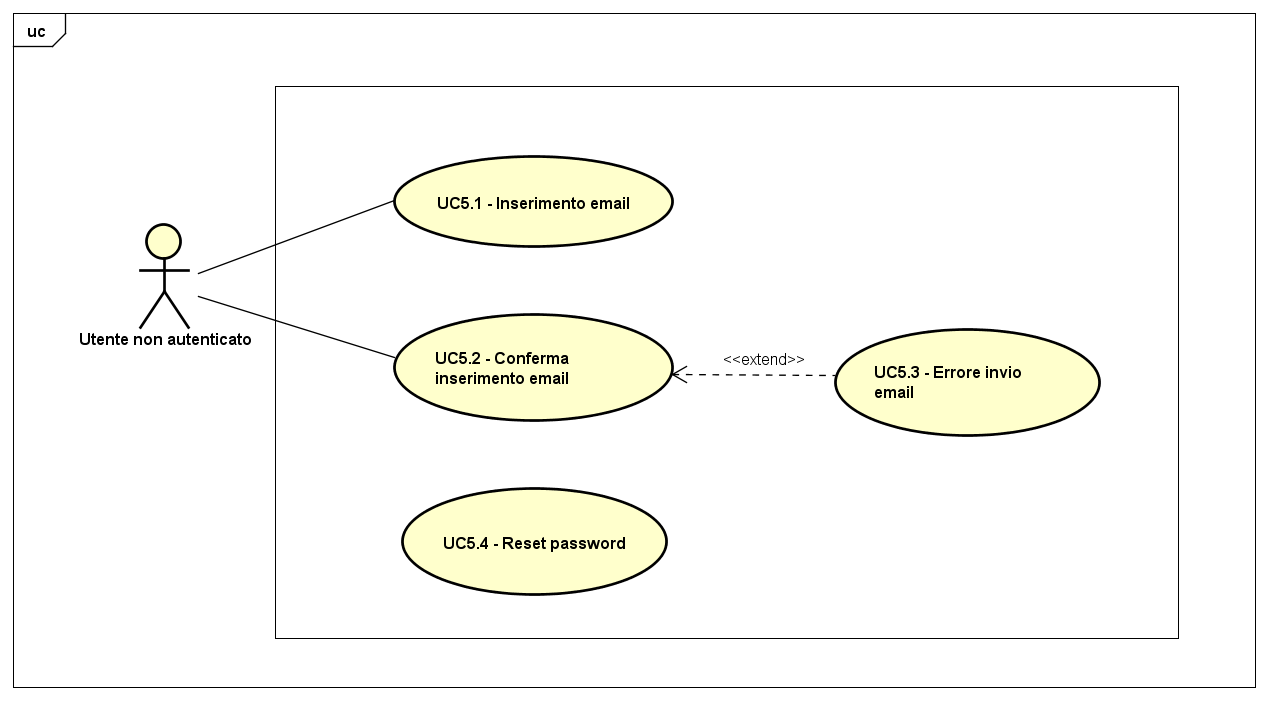
\includegraphics[scale=0.45]{UML/UC5.png}
	\caption{UC5: Recupero Password }
\end{figure}

\begin{longtable}{ l | p{11cm}}
	\hline
	\rowcolor{Gray}
	 \multicolumn{2}{c}{UC5 - Recupero Password} \\
	 \hline
	\textbf{Attori} & Utente Non Autenticato \\
	\textbf{Descrizione} & L'utente non autenticato tenta il recupero della propria password tramite l'invio di una email \\
	\textbf{Pre-Condizioni} & L'utente ha scelto di recuperare la sua password e non è autenticato \\
	\textbf{Post-Condizioni} & L'utente ha ricevuto la propria password tramite una email, oppure la procedura è fallita \\
	\textbf{Scenario Principale} & 
	\begin{enumerate*}[label=(\arabic*.),itemjoin={\newline}]
		\item L'utente non autenticato può inserire la propria email di registrazione (UC5.1)
		\item L'utente non autenticato può confermare l'indirizzo email inserito, al quale l'applicazione web ha inviato la corrispondente password (UC5.2)
	\end{enumerate*}\\
	\textbf{Scenari Alternativi} & 
	\begin{enumerate*}[label=(\arabic*.),itemjoin={\newline}]
		\item L'utente non autenticato visualizza un errore e l'invio della email di recupero password non avviene (UC5.3) 
	\end{enumerate*}\\
\end{longtable}